\documentclass{standalone}
\usepackage{tikz}
\usetikzlibrary{patterns, positioning}

\begin{document}
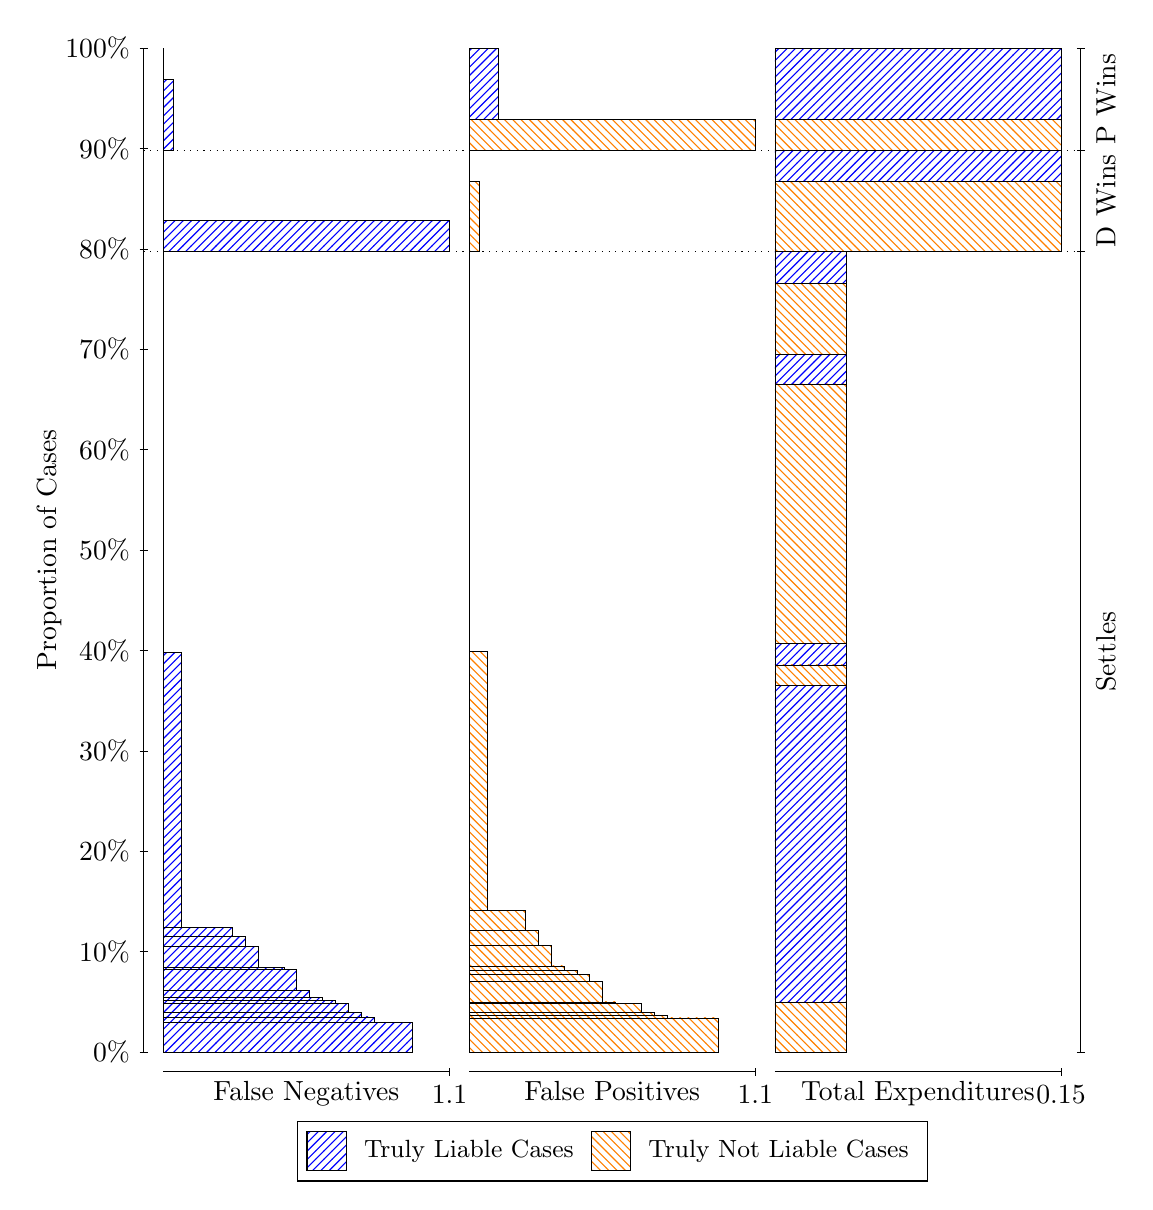
\begin{tikzpicture}
\draw[black, very thin] (1.5,1.75) -- (1.5,14.5);
\node[rotate=90, anchor=center] at (0.3, 8.125) {Proportion of Cases};
\draw[black, very thin] (1.45,1.75) -- (1.55,1.75);
\node[anchor=east] at (1.45, 1.75) {0\%};
\draw[black, very thin] (1.45,3.025) -- (1.55,3.025);
\node[anchor=east] at (1.45, 3.025) {10\%};
\draw[black, very thin] (1.45,4.3) -- (1.55,4.3);
\node[anchor=east] at (1.45, 4.3) {20\%};
\draw[black, very thin] (1.45,5.575) -- (1.55,5.575);
\node[anchor=east] at (1.45, 5.575) {30\%};
\draw[black, very thin] (1.45,6.85) -- (1.55,6.85);
\node[anchor=east] at (1.45, 6.85) {40\%};
\draw[black, very thin] (1.45,8.125) -- (1.55,8.125);
\node[anchor=east] at (1.45, 8.125) {50\%};
\draw[black, very thin] (1.45,9.4) -- (1.55,9.4);
\node[anchor=east] at (1.45, 9.4) {60\%};
\draw[black, very thin] (1.45,10.675) -- (1.55,10.675);
\node[anchor=east] at (1.45, 10.675) {70\%};
\draw[black, very thin] (1.45,11.95) -- (1.55,11.95);
\node[anchor=east] at (1.45, 11.95) {80\%};
\draw[black, very thin] (1.45,13.225) -- (1.55,13.225);
\node[anchor=east] at (1.45, 13.225) {90\%};
\draw[black, very thin] (1.45,14.5) -- (1.55,14.5);
\node[anchor=east] at (1.45, 14.5) {100\%};

\draw[black, very thin] (13.4,1.75) -- (13.4,14.5);
\draw[black, very thin] (13.35,1.75) -- (13.45,1.75);
\node[anchor=west] at (13.35, 1.75) {};
\draw[black, very thin] (13.35,11.918) -- (13.45,11.918);
\node[anchor=west] at (13.35, 11.918) {};
\draw[black, very thin] (13.35,13.201) -- (13.45,13.201);
\node[anchor=west] at (13.35, 13.201) {};
\draw[black, very thin] (13.35,14.5) -- (13.45,14.5);
\node[anchor=west] at (13.35, 14.5) {};

\draw[black, very thin, pattern color=blue, pattern=north east lines] (1.75,1.75) rectangle (4.9139,2.1253);
\draw[black, very thin, pattern color=blue, pattern=north east lines] (1.75,2.1253) rectangle (4.424,2.1967);
\draw[black, very thin, pattern color=blue, pattern=north east lines] (1.75,2.1967) rectangle (4.2607,2.2531);
\draw[black, very thin, pattern color=blue, pattern=north east lines] (1.75,2.2531) rectangle (4.0974,2.3678);
\draw[black, very thin, pattern color=blue, pattern=north east lines] (1.75,2.3678) rectangle (3.9341,2.4082);
\draw[black, very thin, pattern color=blue, pattern=north east lines] (1.75,2.4082) rectangle (3.7708,2.4403);
\draw[black, very thin, pattern color=blue, pattern=north east lines] (1.75,2.4403) rectangle (3.6075,2.533);
\draw[black, very thin, pattern color=blue, pattern=north east lines] (1.75,2.533) rectangle (3.4442,2.8029);
\draw[black, very thin, pattern color=blue, pattern=north east lines] (1.75,2.8029) rectangle (3.2809,2.8283);
\draw[black, very thin, pattern color=blue, pattern=north east lines] (1.75,2.8283) rectangle (2.9543,3.0877);
\draw[black, very thin, pattern color=blue, pattern=north east lines] (1.75,3.0877) rectangle (2.791,3.2221);
\draw[black, very thin, pattern color=blue, pattern=north east lines] (1.75,3.2221) rectangle (2.6277,3.3278);
\draw[black, very thin, pattern color=blue, pattern=north east lines] (1.75,3.3278) rectangle (1.9745,6.8257);
\draw[black, very thin, pattern color=orange, pattern=north west lines] (1.75,6.8257) rectangle (1.75,11.918);
\draw[black, very thin, pattern color=blue, pattern=north east lines] (1.75,11.918) rectangle (5.3833,12.313);
\draw[black, very thin, pattern color=orange, pattern=north west lines] (1.75,12.313) rectangle (1.75,13.201);
\draw[black, very thin, pattern color=blue, pattern=north east lines] (1.75,13.201) rectangle (1.8725,14.105);
\draw[black, very thin, pattern color=orange, pattern=north west lines] (1.75,14.105) rectangle (1.75,14.5);
\draw[black, very thin, pattern color=orange, pattern=north west lines] (5.6333,1.75) rectangle (8.7972,2.1827);
\draw[black, very thin, pattern color=orange, pattern=north west lines] (5.6333,2.1827) rectangle (8.144,2.2132);
\draw[black, very thin, pattern color=orange, pattern=north west lines] (5.6333,2.2132) rectangle (7.9807,2.2518);
\draw[black, very thin, pattern color=orange, pattern=north west lines] (5.6333,2.2518) rectangle (7.8174,2.3678);
\draw[black, very thin, pattern color=orange, pattern=north west lines] (5.6333,2.3678) rectangle (7.4908,2.3848);
\draw[black, very thin, pattern color=orange, pattern=north west lines] (5.6333,2.3848) rectangle (7.3275,2.644);
\draw[black, very thin, pattern color=orange, pattern=north west lines] (5.6333,2.644) rectangle (7.1642,2.7367);
\draw[black, very thin, pattern color=orange, pattern=north west lines] (5.6333,2.7367) rectangle (7.0009,2.7842);
\draw[black, very thin, pattern color=orange, pattern=north west lines] (5.6333,2.7842) rectangle (6.8376,2.8445);
\draw[black, very thin, pattern color=orange, pattern=north west lines] (5.6333,2.8445) rectangle (6.6743,3.101);
\draw[black, very thin, pattern color=orange, pattern=north west lines] (5.6333,3.101) rectangle (6.511,3.2956);
\draw[black, very thin, pattern color=orange, pattern=north west lines] (5.6333,3.2956) rectangle (6.3478,3.5435);
\draw[black, very thin, pattern color=orange, pattern=north west lines] (5.6333,3.5435) rectangle (5.8579,6.842);
\draw[black, very thin, pattern color=blue, pattern=north east lines] (5.6333,6.842) rectangle (5.6333,11.918);
\draw[black, very thin, pattern color=orange, pattern=north west lines] (5.6333,11.918) rectangle (5.7558,12.806);
\draw[black, very thin, pattern color=blue, pattern=north east lines] (5.6333,12.806) rectangle (5.6333,13.201);
\draw[black, very thin, pattern color=orange, pattern=north west lines] (5.6333,13.201) rectangle (9.2667,13.596);
\draw[black, very thin, pattern color=blue, pattern=north east lines] (5.6333,13.596) rectangle (6.0007,14.5);
\draw[black, very thin, pattern color=orange, pattern=north west lines] (9.5167,1.75) rectangle (10.425,2.3848);
\draw[black, very thin, pattern color=blue, pattern=north east lines] (9.5167,2.3848) rectangle (10.425,6.4076);
\draw[black, very thin, pattern color=orange, pattern=north west lines] (9.5167,6.4076) rectangle (10.425,6.6668);
\draw[black, very thin, pattern color=blue, pattern=north east lines] (9.5167,6.6668) rectangle (10.425,6.9367);
\draw[black, very thin, pattern color=orange, pattern=north west lines] (9.5167,6.9367) rectangle (10.425,10.235);
\draw[black, very thin, pattern color=blue, pattern=north east lines] (9.5167,10.235) rectangle (10.425,10.611);
\draw[black, very thin, pattern color=orange, pattern=north west lines] (9.5167,10.611) rectangle (10.425,11.51);
\draw[black, very thin, pattern color=blue, pattern=north east lines] (9.5167,11.51) rectangle (10.425,11.918);
\draw[black, very thin, pattern color=orange, pattern=north west lines] (9.5167,11.918) rectangle (13.15,12.806);
\draw[black, very thin, pattern color=blue, pattern=north east lines] (9.5167,12.806) rectangle (13.15,13.201);
\draw[black, very thin, pattern color=orange, pattern=north west lines] (9.5167,13.201) rectangle (13.15,13.596);
\draw[black, very thin, pattern color=blue, pattern=north east lines] (9.5167,13.596) rectangle (13.15,14.5);
\draw[black, dotted] (1.5,11.918) -- (13.4,11.918);
\draw[black, dotted] (1.5,13.201) -- (13.4,13.201);
\draw[black, very thin] (1.75,1.5) -- (5.3833,1.5);
\node[anchor=north] at (3.5667, 1.5) {False Negatives};
\draw[black, very thin] (5.3833,1.45) -- (5.3833,1.55);
\node[anchor=north] at (5.3833, 1.45) {1.1};

\draw[black, very thin] (5.6333,1.5) -- (9.2667,1.5);
\node[anchor=north] at (7.45, 1.5) {False Positives};
\draw[black, very thin] (9.2667,1.45) -- (9.2667,1.55);
\node[anchor=north] at (9.2667, 1.45) {1.1};

\draw[black, very thin] (9.5167,1.5) -- (13.15,1.5);
\node[anchor=north] at (11.333, 1.5) {Total Expenditures};
\draw[black, very thin] (13.15,1.45) -- (13.15,1.55);
\node[anchor=north] at (13.15, 1.45) {0.15};

\node[black, centered, rotate=90] at (13.72, 6.8339) {Settles};
\node[black, centered, rotate=90] at (13.72, 12.559) {D Wins};
\node[black, centered, rotate=90] at (13.72, 13.85) {P Wins};

\draw (7.449999999999999,1.5) node[draw=none] (baseCoordinate) {};
\begin{scope}[align=center]
        \matrix[scale=0.5, draw=black, below=0.5cm of baseCoordinate, nodes={draw}, column sep=0.1cm]{
            \node[rectangle, draw, minimum width=0.5cm, minimum height=0.5cm, pattern=north east lines, pattern color=blue] {}; &
            \node[draw=none, font=\small] (B) {Truly Liable Cases}; &
            \node[rectangle, draw, minimum width=0.5cm, minimum height=0.5cm, pattern=north west lines, pattern color=orange] {}; &
            \node[draw=none, font=\small] (B) {Truly Not Liable Cases}; \\
            };
\end{scope}

\end{tikzpicture}
\end{document}